\subsection{Database Design}
	The current model that was provided with the current build of CAMEL will be used with the same naming structure, except additional modifications will be made with some models along with new models will be added. Changes to the current models will be done to ensure that additional functionality can work correctly. One example of the change that occurred was the introduction of a new parser into CAMEL. This parser modifies the BookNode model by removing Mpath. The main aim of the changes to the database it to ensure compatibility with newer functionality, though it will not have a large impact for usability with the new system.\\
	
	The models that will be included in CAMEL will be:
	\begin{itemize}
		\item \textbf{BookNode}: This object relates to different Latex components that make up the whole document. Each BookNode contains a parent node, unless is the root node which remains null. Each node has a parent as it allows it to be accessed by Django - MPTT when traversing through the nodes to generate a page. The BookNode is used in other tables to link the page together.     
		
		\item \textbf{TextNode}: Each TextNode contains the text that was contained inside latex markup. These objects will contain the relevant information that will be outputted by Django - MPTT when renders the relevant HTML during the web page rendering process. Each TextNode has a parent BookNode, which contains the location for it.  
		
		\item \textbf{Book}: This is the object that will provide a connection between the BookNode object and the Module object. This allows modules to select which books are relevant and add them to the list that the student can access to study from and complete tasks on. The Book object will take a 'root' (start of latex book) BookNode object to allow the connection. 
		
		\item \textbf{Module}: This object relates to the module a student will take. It will contain the current year of study and provides a link for students to access relevant books and tasks that are required to be completed. Each module will contain a number of relevant books for them to study from.
		
		\item \textbf{Submission}: The submission object will be used to submit all answers that a student has entered from objects 'SingleChoiceAnswer' and 'Answer.' With each of these submissions, it will not allow a lecturer to access any of their details, such as their name. This allows the submissions to keep with university policy concerning anonymous marking. A student can only submit a quiz or homework once from each chapter in a book.   
		
		\item \textbf{SingleChoiceAnswer}: This object is used to hold the answers from the multiple choice questions that are on CAMEL. This object allows the student to save and comeback later to the question and continue. The answer is stored within and is used with 'Submission' to allow a student to submit their answers. 
		
		\item \textbf{Answer}: Answer is the object that is used to store the answer from a question where a range of answers can be entered via a input box. This will hold any latex that the student enters and can be viewed in the question on the UI side. This also will be used to save the answer for submission. Like 'SingleChoiceAnswer,' the answer entered can be saved and question can be continued later on. 
	\end{itemize}
	
	We will also be utilising some pre-existing tables that have been included with Django. One of these is Users which is the backbone of creating the Students, Administrator and Lecturer accounts. We have decided to use this table as it provides much of the functionality that we need in terms of security that could take some time to implement ourselves. For example, restrictions can be easily applied as Django has already provided this functionality. Additionally, security is greater with using User as Django has also provided a 'hash and salt' hashing mechanism in the table to protect user passwords. By using Django tables, much of our time can be focused on development and we can guarantee that the data is secure which is important to any institution.\\	
	
	\begin{figure}[h]
		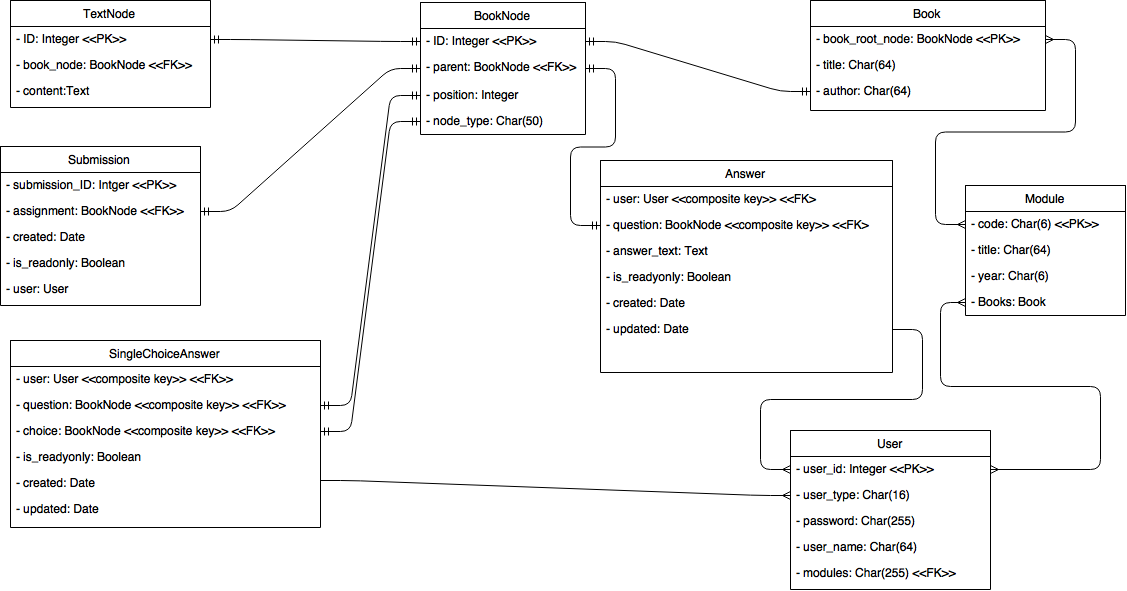
\includegraphics[scale=0.45]{implementation/img/database_design}
		\caption{CAMEL Database Design}
	\end{figure}